\documentclass[12pt,a4paper,twoside]{article}
\usepackage[utf8]{inputenc}
\usepackage[spanish]{babel}
\usepackage{amsmath}
\usepackage{amsfonts}
\usepackage{amssymb}
\usepackage{graphicx}
\usepackage[left=2cm,right=2cm,top=2cm,bottom=2cm]{geometry}
\author{Yoleivys Delgado}
\title{\textbf{Movimiento de translación de la Tierra}}
\begin{document}
\maketitle
El movimiento traslacional de la tierra, es la trayectoria a lo largo de la cual la Tierra viaja alrededor del sol. La distancia promedio entre la tierra y el sol es de $149,000.000 Km$ y una orbita completa toma alrededor de 365.26 días.\\
Para la realización de este práctica supondremos que la tierra gira alrededor del sol con un \textbf{movimiento circular uniforme } a adistancia fija del sol de $R = 1.49 . 10^{8} Km $.
Recordemos que un movimiento circular uniforme describe el movimiento de un cuerpo a través de una ruta circular con velocidad constante.\\
Para un movimiento circular uniforme de radio R, periodo T y velocidad angular $\omega$ tenemos:
\begin{eqnarray}
\omega = \frac{2 \pi}{T} = \frac{d\theta}{dt}.
\end{eqnarray}
La grafica optenida de esta practica como los codigos fortran y gnuplot con mostrados en las figuras (\ref{fig:figura1}),(\ref{fig:figura2}) y (\ref{fig:figura3}) . 
\newpage
\begin{figure}[h]
\centering
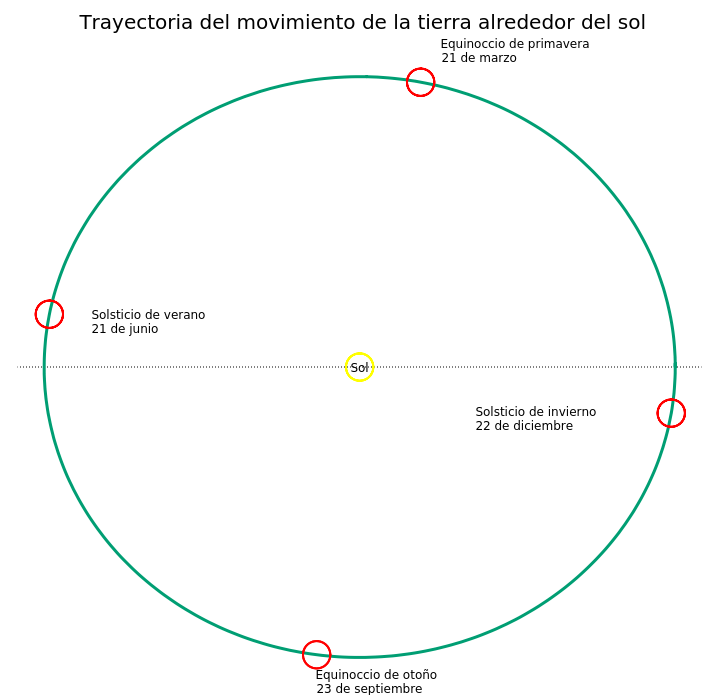
\includegraphics[width=10cm]{imagen.png} 
\caption{Trayectorias del movimiento de la Tierra alrededor del Sol}
\label{fig:figura1}
\end{figure}
\newpage
\begin{figure}[h]
\begin{verbatim}
set title 'Trayectoria del movimiento de la tierra alrededor del sol'
set title font ",15" norotate
set style data lines      # Todas las graficas las pone con lineas
set xzeroaxis
unset key
unset border
unset xtics
unset ytics
set xrange [-162000000.0:162000000.0]
set yrange [-162000000.0:162000000.0]
set label 1 "Sol" at 0.0, 0.0 center front
set label 2  at  38934692.676988836, 166775146.26014927
set label 2 "Equinoccio de primavera\n21 de marzo" 
set label 3  at  -127105887.13936114, 27203271.291180104
set label 3 "Solsticio de verano\n21 de junio"  
set label 4  at  -20382310.488603789, -158204997.95602763
set label 4 "Equinoccio de otoño\n23 de septiembre" 
set label 5  at  54770601.2, -22729338.9
set label 5 "Solsticio de invierno\n22 de diciembre" 
plot "Mov_tierra.txt" using 2:3 ls 2 lw 3,\
"posicion.txt" using 2:3 with circles lw 2 lc rgb "red",\
"Sol.txt" using 2:3 with circles lw 2 lc rgb "yellow"
\end{verbatim}
\caption{Codigo gnuplot de la gráfica de la figura 1}
\label{fig:figura2}
\end{figure}

\begin{figure}[h]
\begin{verbatim}
function funcx (a)
  ! Esta funcion permite onterner la posicion en x de la tierra alrededor del sol
  ! en coordenadas rectangulares.
  implicit none 
  double precision :: funcx
  double precision, intent (in) :: a  ! ángulos barridos 
  double precision, parameter :: R=1.496d8 ! R es el radio de la tierra 
  
  funcx = R * dcos(a)
  
end function funcx
!***********************************************************************************
function funcy (a)
  ! Esta funcion permite onterner la posicion en y de la tierra alrededor del sol
  ! en coordenadas rectangulares.
  implicit none 
  double precision :: funcy
  double precision, intent (in) :: a
  double precision, parameter :: R=1.496d8
  
  funcy = R * dsin(a)
  
end function funcy
!************************************************************************************
program movi_tierra
  implicit none
  integer :: i
  double precision :: a, funcx, funcy
  double precision, parameter :: R=1.496d8, pi=3.141592d0, T=365.26d0
  double precision, dimension(0:366):: x,y,dt, dteta

  open (1, file='Mov_tierra.txt', status= 'unknown')

  do i=0,366
     
     dt(i) = dble (i)
     
     ! intervalo de ángulo
     dteta(i) = (2.0d0*180.0d0*dt(i))/T
     
     ! convertir grados a radianes
     a = (dteta(i)*pi)/180.0d0

     ! llamando funciones
     x(i) = funcx (a)
     y(i) = funcy (a)

     write (1,*)  dt(i), x(i), y(i)

  end do

  close (1)

end program movi_tierra
\end{verbatim}
\caption{Codigo gnuplot de la gráfica de la figura 1}
\label{fig:figura3}
\end{figure}
\end{document}
